\chapter{Stanowisko demonstracyjne}
\label{cha:stanowiskodemonstracyjne}

Pierwszą częścią pracy jest skompletowanie stanowiska demonstracyjnego, w skład którego wchodzą:
\begin{itemize}
	\item Kamera
	\item Platforma obliczeniowa
	\item Serwomechanizmy
	\item Sterownik serwomechanizmów
	\item Zasilanie
	\item Wskaźnik
\end{itemize}

\section{Kamera}
\label{sec:kamera}

Postanowiono użyć kamery\dots(Tutaj nazwa kamery, specyfikacja, krótki opis).

\section{Platforma obliczeniowa}
\label{sec:platformaobliczeniowa}

\begin{figure}[H]
	\centering
	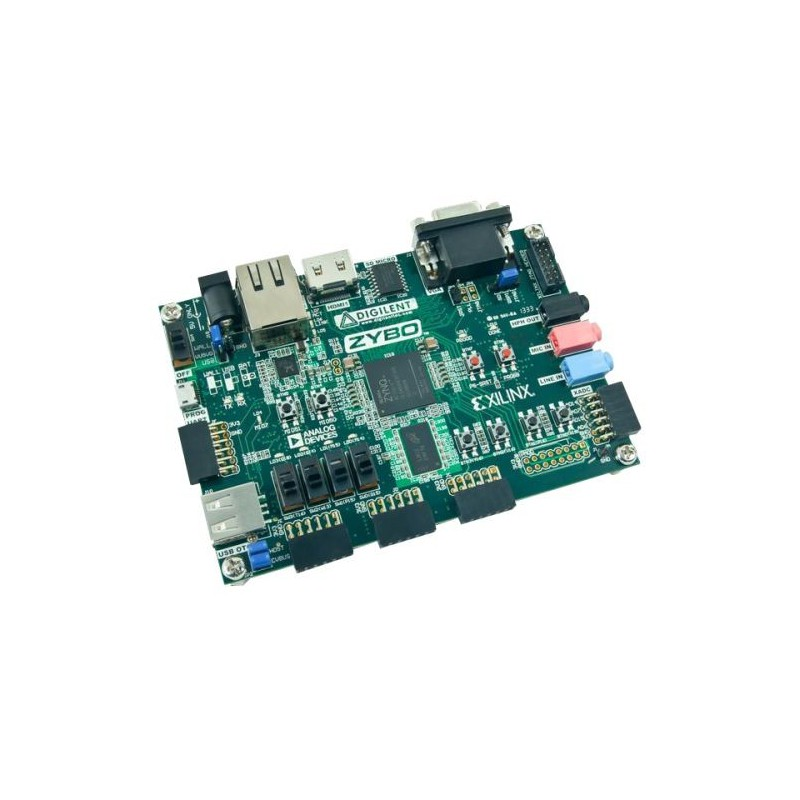
\includegraphics[width=4in]{zybo.jpg}
	%\caption{\label{fig:zybo}Płytka ZYBO Zynq-7000.}
	\captionsource{Płytka ZYBO Zynq-7000.}{\cite{Xi}}
\end{figure}

Zdecydowano, że platformę obliczeniową stanowić będzie płytka ZYBO. Jest to bogato wyposażone narzędzie zawierające układ programowalny z rodziny Xilinx Zynq-7000. Układ ten oparty jest na architekturze Xilinx All Programable System-on-Chip, w której zintegrowany został dwurdzeniowy procesor ARM Cortex-A9 i układ programowalny FPGA z serii Xilinx 7. Zawiera ona m.in. port HDMI potrzebne do odbieranie obrazu z kamery oraz port VGA, który umożliwia nam wysyłanie obrazu do monitora \cite{Xi}. W układzie programowalnym zaimplementowany zostanie tor wizyjny przetwarzający potokowo dane przesyłane z kamery oraz wyznaczający położenie obiektu w danej ramce. Oprócz tego musi on komunikować się ze sterownikiem serwomechanizmów w celu pozycjonowania głowicy w wyznaczonym punkcie oraz z komputerem klasy PC, aby otrzymywać parametry pracy oraz ustawiać początkową pozycję głowicy.

\section{Serwomechanizmy}
\label{sec:serwomechanizmy}

Ruchomą głowicę postanowiono skonstruować wykorzystując serwomechanizmy dostępne na rynku. Przy wyborze brano pod uwagę serwomechanizmy analogowe, serwomechanizmy cyfrowe oraz serwomechanizmy smart.

\subsection{Serwomechanizm analogowy}
Serwomechanizm ten sterowany jest impulsami podawanymi z częstotliwością 50 Hz. Podawanie impulsów z większą częstotliwością może doprowadzić do uszkodzenia urządzenia. W zależności od czasu trwania impulsu serwomechanizm ustawia się w odpowiedniej pozycji i ją utrzymuje. Kontrola położenia odbywa się za pomocą potencjometru sprzężonego z kołem zębatym. Serwomechanizm tego typu nie reagują szybko i nie produkują wystarczającego momentu kiedy zadajemy małe przesunięcie.

\subsection{Serwomechanizm cyfrowy}
Jest on, podobnie jak serwomechanizm analogowy, sterowany impulsami. Podawać można je jednak z maksymalną częstotliwością powyżej 300 Hz. W porównaniu do serwomechanizmu analogowego przyspiesza ono szybciej i produkuje stabilniejszy moment obrotowy. Reagują również lepiej na polecenia małych zmian pozycji. Z drugiej strony  potrzebują one dużo większej mocy. Prąd, który pobierają w trakcie pracy, może sięgać kilku amperów.

\subsection{Serwomechanizm smart}
Główną różnicą pomiędzy serwomechanizmami standardowymi, a smart, jest sposób komunikacji w celu podania wartości zadanej położenia. Zamiast impulsów o różnej szerokości wykorzystuje się komunikację szeregową. Ich obsługa jest więc bardziej skomplikowana. Najpopularniejszymi protokołami są TTL Half-Duplex, TTL Full-Duplex i RS-485. Za pomocą komunikacji tego typu można zmieniać dużo więcej parametrów niż tylko pozycję zadaną. Można zmieniać nastawy regulatora PID, maksymalną prędkość kątową lub maksymalny moment. W przeciwieństwie do serwomechanizmów klasycznych, możemy również odczytywać aktualną pozycję serwomechanizmu. Minusem tych urządzeń jest ich cena oraz dostępność. Są one kilka razy droższe od cyfrowych serwomechanizmów o podobnych parametrach.

\paragraph*{}
Postanowiono użyć dwóch serwomechanizmów cyfrowych PowerHD D-21HV. Są to serwomechanizmy typu standard o dużym momencie obrotowym i wysokiej maksymalnej prędkości obrotowej. Wyposażone jest w łożyska kulkowe oraz tytanowe tryby w celu zwiększenia jego wytrzymałości. Specyfikacja serwomechanizmów:
\begin{itemize}
\item Napięcie zasilania: \(6.0-7.4\) V
\item Zakres ruchu: \(155^\circ\)
\item Masa: \(75\) g
\item Moment: \(21\) kg\(\cdot\)cm dla napięcie \(7.4\) V
\item Prędkość: \(0.12\)s/\(60^\circ\) dla napięcia \(7.4\) V
\end{itemize}
\paragraph*{}
Urządzenia te mogą pobierać impulsowy prąd o wartości nawet powyżej 3 A. Sterowane są za pomocą impulsów podawanych z częstotliwością 333 Hz. Pozycję naturalną zadajemy podając impulsy o czasie trwania \(1500 \mu\)s. Serwa zostały połączone w głowicę za pomocą metalowych uchwytów dedykowanych do łączenia serwomechanizmów typu standard w konfigurację PT.

\section{Sterownik serwomechanizmów}
\label{sec:sterownik}

\begin{figure}[h]
	\centering
	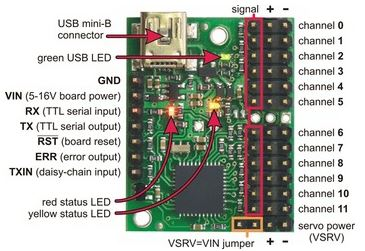
\includegraphics[width=4in]{maestro.jpg}
	\captionsource{Sterownik serwomechanizmów Pololu Mini Maestro.}{\cite{MM}}
\end{figure}

Do sterowania serwomechanizmami postanowiono użyć gotowego sterownika produkowanego przez firmę Pololu. 12-kanałowy sterownik Mini Maestro pozwala na równoczesną obsługę obu serwomechanizmów. Oprócz podawania wartości zadanej w postaci impulsów pozwala on również na zmianę ustawianie maksymalnej prędkości obrotowej i maksymalnego momentu obrotowego. Dzięki temu możemy dużo lepiej kontrolować urządzenia wykonawcze i zapewnić bardziej ciągły ruch głowicy. Komunikujemy się z nim za pośrednictwem interfejsu szeregowego UART z prędkością 115200 bitów na sekundę.

\section{Zasilanie}
\label{sec:zasilanie}
Do zasilania głowicy użyty został zasilacz impulsowy Redox, który na wyjściu daje napięcie 12 V i maksymalny prąd 5 A. Jako, że serwomechanizmy potrzebują napięcia 7.4 V używamy przetwornicy step-down XL4005E1 o regulowanym napięciu wyjściowym. Maksymalny prąd wyjściowy użytej przetwornicy wynosi 5 A. Zdecydowanie wystarczy to do zasilenia użytych serwomechanizmów.

\section{Wskaźnik}
\label{sec:wskaznik}

Postanowiono użyć zwykłego wskaźnika laserowego do wskazywania miejsca, w stronę którego zwrócona jest głowica.